\section{Mass Hanging from a Spring (3D)}

Consider a 3D system with a point mass $m$ hanging from a fixed point (which is treated as the origin in the coordinate system chosen for this problem) via a spring of a spring constant $k$ and null rest length $l_0 = 0$.

Let $\vec{x}$ be the position vector of the mass, and $\vec{T}$ be the tensile force exerted on the mass by the spring. One can thus assert that

\begin{equation}
    T = kx
\end{equation}

and

\begin{equation}
    \hat{T} = - \hat{x}.
\end{equation}

\subsection{Linear Solutions}
With a rest length of $l_0 = 0$, the equations of motion are linear and can be decomposed into the forms

\begin{align}
    \ddot{x} &= \omega_0^2 x \\
    \ddot{y} &= \omega_0^2 y + g\\
    \ddot{z} &= \omega^2 z
\end{align}

all of which have analytical solutions that can be written with trigonometric functions, which is indicative of periodic motion. This can be double-checked with numerical solutions.

\begin{figure}
    \centering
    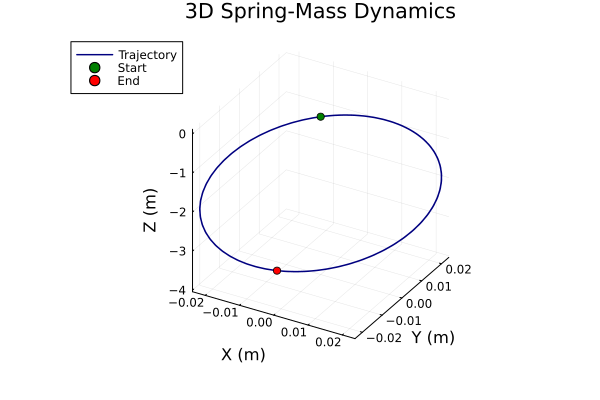
\includegraphics[width=0.75\textwidth]{Problems/Problem10/figures/linear.png}
    \caption{Generic Solution of the System with $l_0 = 0$ (linear)}
\end{figure}

\subsection{Non-Linear Solutions}

The equations of motion with a non-zero spring rest-length are

\begin{equation}
    m\ddot{\vec{x}} = \frac{k}{m} (x - l_0)\cdot \frac{x}{\sqrt{x^2 + y^2+ z^2}} - g\hat{y}
\end{equation}

where $x = \sqrt{x^2 + y^2 + z^2}$. These terms cancel out if $l_0 = 0$. On the contrary, if $l_0 \neq 0$, non-linearity is preserved by the $\sqrt{x^2 + y^2 + z^2}$ term.

Solving this system numerically, non-linear behavior is observed.

\begin{figure}
    \centering
    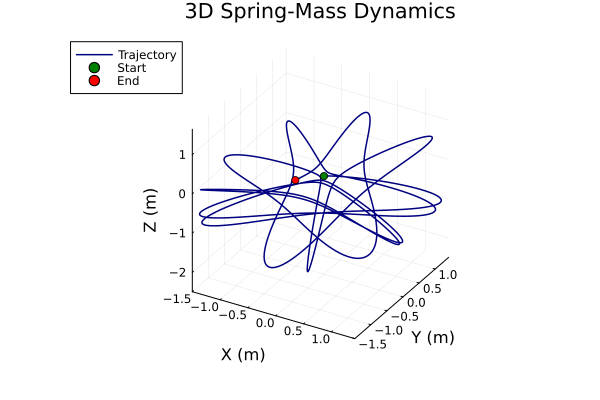
\includegraphics[width=0.75\textwidth]{Problems/Problem10/figures/non_linear_L0.png}
    \caption{Generic non-linear behavior $l_0 \neq 0$}
\end{figure}




